%%%%%%%%%%%%%%%%%%%%%%%%%%%%%%%%%%%%%%%%%%%%%%%%%%%%%%%%%%%%%%%%%%%%%%%%
%                                                                      %
%     File: Thesis_Background.tex                                      %
%     Tex Master: Thesis.tex                                           %
%                                                                      %
%     Author: Andre C. Marta                                           %
%     Last modified :  2 Jul 2015                                      %
%                                                                      %
%%%%%%%%%%%%%%%%%%%%%%%%%%%%%%%%%%%%%%%%%%%%%%%%%%%%%%%%%%%%%%%%%%%%%%%%

\chapter{Investing and entering the market with a new product}
\label{chapter:background}

Insert your chapter material here...


%%%%%%%%%%%%%%%%%%%%%%%%%%%%%%%%%%%%%%%%%%%%%%%%%%%%%%%%%%%%%%%%%%%%%%%%
\section{Introduction}
\label{section:overview}

Situação do problema.
Trabalhos já realizados e de maneira os extendemos.

Some overview of the underlying theory about the topic...


%%%%%%%%%%%%%%%%%%%%%%%%%%%%%%%%%%%%%%%%%%%%%%%%%%%%%%%%%%%%%%%%%%%%%%%%
\section{Stopping Problem}
\label{section:1_theory}



\subsection{Benchmark Model}
\label{subsec:1_bm}

\subsection{Capacity Optimization Model}
\label{subsec:1_com}



\section{Maximization Problem}
\label{section:1_probmax}


Having calculated the expression of optimized value function $F^*$, our goal now is to calculate the optimal level of investment $R$, taking into account that it influences the waiting time for the breakthrough to happen. In order to do it, we need to maximize the expected value of the optimized value function.

Notice that the distribution of the waiting time is given by an Exponential with parameter $\lambda(R)$. Also, since we are interested to find the optimal level of investment made now, one may not forget to discount the optimized value function.
Thus we obtain that our optimal level of investment leads to a value function given by 


\begin{align*}
V(x) &=\max_R E \left[ e^{-rt} F^*(x) -R \right]\\
& =  \max_R  \left\{ \int_0 ^\infty \lambda(R) e^{-\lambda(R)t} e^{-rt} F^*(x) dt -R \right\} \\
% &=\max_R E \left[ e^{-rt} \sup_\tau E ^{X_0=x}\left[\max_K e^{-r\tau}h(X_\tau,K) 1_{\{\tau<\infty\}} \right]dt - R \right] \\
&= \max_R \left\{ \int_0 ^\infty \lambda(R) e^{-\lambda(R)t} e^{-rt} 
\sup_\tau E ^{X_0=x}\left[\max_K e^{-r\tau}h(X_\tau,K) 1_{\{\tau<\infty\}} \right]
dt -R \right\} \\
&= \max_R \left\{  \int_0 ^\infty \lambda(R) e^{-(\lambda(R)+r)t} \frac{(\theta x -\delta (r-\mu))^2}{4 \alpha (r-\mu) x} -R \right\}
\end{align*}




Since $F^*(x)$ does not depend on investment $R$ nor time $t$, and it only depends on the drift $\mu$, the volatility $\sigma$ of GBM, discount rate $r$, innovation level after the jump $\theta$ and sensibility parameters $\alpha$ and $\delta$ and noticing that $R^\gamma+r>0$, since we have no negative investment, we obtain
$$ V(X) =\max_R \left\{ \frac{R^\gamma}{R^\gamma+r} F^*(x) -R \right\}.$$

The optimal value of the investment to make, $R^*$, is found by analyzing the first and the second partial derivatives of the expression to maximize.

\begin{align*}
\frac{\partial}{\partial R} \left( \frac{R^\gamma}{R^\gamma+r} F^*(x) -R \right) &= \frac{\gamma R^{\gamma-1}F^*(x)r-(R^\gamma+r)^2}{(R^\gamma+r)^2}\\
\frac{\partial^2}{\partial R^2} \left( \frac{R^\gamma}{R^\gamma+r} F^*(x) -R \right) &=
-\frac{F^*(x) \gamma r R^{-2+\gamma}(r-\gamma r+(1+\gamma)R^\gamma)}{(R^\gamma+r)^3}
\end{align*}



\subsection{Case I: $\gamma=1 \Leftrightarrow \lambda(R)=R$}

Analysing the roots of the first partial derivative in order to parameter $R$, we get a quadratic polynomial for which we can calculate obtain the expression of the zeros, obtaining
%$$   \frac{\partial}{\partial R} \left( \frac{R}{R+r} F(X) -R \right) = \frac{ F(X)r-(R+r)^2}{(R+r)^2}=0 $$

%$$   \Rightarrow F(X)r-(R^2+2rR+r^2)=0$$
$$  R=-\sqrt{F^*(X)r}-r \  \vee \ R=\sqrt{F^*(X)r}-r$$



The first solution is not admissible, since it's not possible to have negative investment. Thus, we only have to check if $R=\sqrt{F(x)r}-r$ corresponds to a minimum or a maximum. To do that, we analyse the second partial derivative as stated above.

$$\frac{\partial^2}{\partial R^2} \left( \frac{R}{R+r} F(x) -R \right) 
% =    -\frac{F(X) r R^{-1}(r-r+2R)}{(R+r)^3}
= -\frac{2rF^*(x)}{(R+r)^3}<0$$
where we used the fact that $R,\ r, \ F(x)>0$.

We get then that, in order to have
$$ \text{arg} \max_R V(x)= \sqrt{F^*(x)r}-r $$
we need to verify
\begin{equation}
F(x)>r
\label{ass3}
\end{equation}

\subsection{Case II: $\gamma \in (0,1) $}
Since the second derivative is negative for considered values of $\gamma$ and $r,R>0$, any positive root of the first partial derivative in order to $R$ accomplishes our goal of maximizing the expression above.

When analyzing the roots of the first derivative we obtain the following polynomial, 

$$
%\frac{\partial}{\partial R} \left( \frac{R^\gamma}{R^\gamma+r} F(X) -R \right) = \frac{\gamma R^{\gamma-1}F(X)r-(R^\gamma+r)^2}{(R^\gamma+r)^2}=0 \quad \Rightarrow \quad 
R^{\gamma-1}F^*(x)r-R^{2\gamma}-2rR^\gamma-r^2=0,$$

which unfortunately, we are not able to solve analytically for every value $\gamma \in (0,1) $. We considered some numerical illustrations for values $\gamma \in (0,1)$ presented in Section \ref{subsec:RDcap1}.




\section{Comparative Statics}

\subsection{Benchmark and Capacity Optimization Model}
efeitos de $\mu, \ \sigma, \ \delta$.
In this section we study the behaviour of the decision threshold $x^*_B$ and $x^*_{C}$ and $K^*$ as described in \eqref{label}, with
the different parameters.

Comparisons between the benchmark and capacity optimization models will be made.\\
\textbf{Proposition:}
Decision thresholds $x^*_B$ and $x^*_{C}$ increase with $ \sigma, \ \delta$, decrease with $\theta$ and do not have a monotonic behaviour with $\mu$.


\textbf{Proof:}
First note that $x^*_B$ increases with $K$ and it verifies $\lim \limits_{K \to 0} x^*_B(K)=x^*_{C}$, $\lim \limits_{K \to \theta/\alpha} x^*_B(K)=\infty$ and that $\forall K \in [0, \theta/\alpha): x^*_B(K)\geq x^*_{C}$, where $\theta/ \alpha$ is considered to be the maximum value that the capacity can take due to restriction MENCIONAR. Thus $x^*_C$ is a particular case of $x^*_B$. Since the capacity does not depend on the other parameters, we have that results that hold for $x^*_B$, will also hold for $x^*_C$. 

Regarding $\sigma$, we observe that

     $$    \frac{\partial x^*_B ( \sigma ) }{\partial \sigma}= 
\frac{16 \delta (r-\mu) \left(2 \mu ^2-\mu  \sigma ^2 \left(\sqrt{\frac{4 \mu ^2}{\sigma ^4}-\frac{4 \mu }{\sigma ^2}+\frac{8 r}{\sigma ^2}+1}+1\right)+2 r \sigma ^2\right)}{\sigma  (\theta-\alpha K) \sqrt{\frac{4 \mu ^2}{\sigma ^4}-\frac{4 \mu }{\sigma ^2}+\frac{8 r}{\sigma ^2}+1} \left(\sigma ^2 \left(\sqrt{\frac{4 \mu ^2}{\sigma ^4}-\frac{4 \mu }{\sigma ^2}+\frac{8 r}{\sigma ^2}+1}-1\right)-2 \mu \right)^2}>0$$

The numerator is positive since, using the fact that $r>0 \Rightarrow 2r>r$, and $r-\mu>0$, it follows that
\begin{equation}
2 \mu ^2-\mu  \sigma ^2 \left(\sqrt{\frac{4 \mu ^2}{\sigma ^4}-\frac{4 \mu }{\sigma ^2}+\frac{8 r}{\sigma ^2}+1}+1\right)+2 r \sigma ^2 \
\geq \ 2 \mu ^2-\mu  \sigma^2+ 2r \sigma ^2 \ 
= \  2 \mu ^2+ \sigma^2 (2 r-\mu) \ > \ 2 \mu ^2+ \sigma^2 (r-\mu) >0.
\label{demo}
\end{equation}

On the other side, the denominator is positive (and real) since all its expressions are positive. In particular $\sqrt{\frac{4 \mu ^2}{\sigma ^4}-\frac{4 \mu }{\sigma ^2}+\frac{8 r}{\sigma ^2}+1}>0$.
This can be showed using the fact that $d_1=\frac{1}{2}-\frac{\mu}{\sigma^2} +\sqrt{\left( \frac{1}{2} -\frac{\mu}{\sigma^2} \right) ^2+ \frac{2r}{\sigma^2}}>1$. Manipulating the expression we obtain that
\begin{equation}
 d_1-\frac{1}{2}+\frac{\mu}{\sigma^2}= \sqrt{ \frac{\mu^2}{\sigma^4}-\frac{\mu}{\sigma^2} +\frac{2r}{\sigma^2}+\frac{1}{4} }>0,
 \label{condd1}
\end{equation}
 since $d_1-\frac{1}{2}>\frac{1}{2} \Rightarrow d_1-\frac{1}{2}+\frac{\mu}{\sigma^2}>0$, for values of $\mu$ and $\sigma$ such that $\mu>\left( \frac{1}{2}-d_1 \right) \sigma^2$. Thus, by multiplying the square root in \eqref{condd1} by 4, we obtain  $\sqrt{\frac{4 \mu ^2}{\sigma ^4}-\frac{4 \mu }{\sigma ^2}+\frac{8 r}{\sigma ^2}+1}$, from which our result holds.
 
 
 Regarding $\delta$, since $d_1$ doesn't depend on $\delta$, it follows that
 \begin{align*}
 \frac{\partial x^*_B (\delta)}{\partial \delta}= \frac{d_1}{d_1-1} \frac{\delta (r-\mu)}{\theta-\alpha K}>0,
 \end{align*}
 
 
 Regarding $\theta$, we observe that if its value increases, the denominator of $x^*_B$ increases leading $x^*_B$ to decrease.
 
 Regarding $\mu$, we obtain that
 \begin{align*}
 \frac{\partial x^*_B (\mu)}{\partial \mu}=\frac{\sqrt{\sigma^4+4 \mu^2 -4 \mu\sigma^2+8r\sigma^2}(\sigma^2-2\mu)\delta}{(\sigma^4+4 \mu^2 -4 \mu\sigma^2+8r\sigma^2)(\theta-\alpha K )} =
 \begin{cases}
 <0 &\ \text{for} \ \mu<\frac{\sigma^2}{2}\\
 >0 &\ \text{for} \ \mu>\frac{\sigma^2}{2}
 \end{cases}.
 \end{align*}
 
 From \eqref{condd1}, and in a similar way as previously done, we obtain that
 $$2 \sigma^2 \sqrt{ \frac{\mu^2}{\sigma^4}-\frac{\mu}{\sigma^2} +\frac{2r}{\sigma^2}+\frac{1}{4} }= \sqrt{ \sigma^4+4 \mu^2 -4 \mu\sigma^2+8r\sigma^2}>0$$
 and that $\sigma^4+4 \mu^2 -4 \mu\sigma^2+8r\sigma^2>0$. Then we have that, holding condition CONDICAO, the denominator is positive. Since $\delta>0$, the non-monotone behaviour, represented above, comes for the region where $\sigma^2-2\mu$ is negative and positive, respectively. Note that we obtain that $\mu=\frac{\sigma^2}{2}$ is a stationary point, where the minimum value of $x^*_B$ is observed.
 
 
 
 
\begin{flushright}
 $\square$
\end{flushright}



To illustrate results above mentioned we performed some numerical illustrations, using software \textit{Mathematica} and its function \texttt{Manipulate}. However here are only able to present static plots - we leave to the interested ones, to see the results achieved with \texttt{Manipulate}.

Unless it is written the opposite, following values were considered:


\begin{table*}[!htb]
	\centering
	%\label{my-label}
	\begin{tabular}{lllllll}
		 $\bullet$ & $\mu=0.03$     &  & \hspace{7cm} &  &  $\bullet$ & $\alpha=0.01$ \\
		 $\bullet$ & $\sigma=0.005$ &  & \hspace{7cm} &  &  $\bullet$ & $\theta=10$   \\
		 $\bullet$ & $r=0.05$       &  & \hspace{7cm} &  &  $\bullet$ & $K=100$       \\
		 $\bullet$ & $\delta=2$     &  & \hspace{7cm} &  &                                    
	\end{tabular}
%\caption{bjde}
\end{table*}

%\begin{itemize}
%		\item $\mu=0.03$
%		\item $\sigma=0.005$ 
%		\item $r=0.05$
%		\item $\delta=2$
%		\item $\alpha=0.01$
%		\item $\theta=10$
%		\item $K=100$	
%\end{itemize}


We start by illustrating how does $x^*_B$ and $x^*_C$ are related by the capacity level $K$, on which $x^*_B$ is dependent. One can see on Figure \ref{fig:Kvar} that conclusions mentioned on the proof (including that $x^*_B(0)=x^*_C$) hold.

\begin{figure}[!htb]
	\centering
	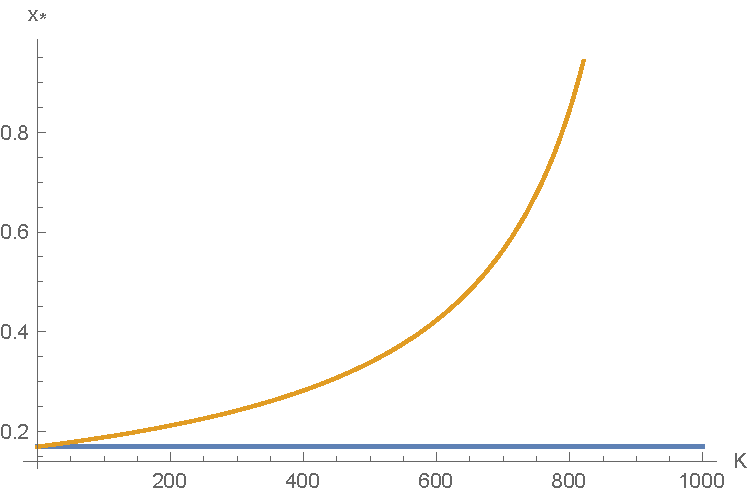
\includegraphics[width=0.45\textwidth]{Prob1_CapOpt/xopt_kvar.pdf}
	\caption{Threshold value with respect to the benchmark model (orange) and the capacity optimized model (blue), considering capacity levels $K \in [0, \theta/\alpha)$.}
	\label{fig:Kvar}
\end{figure}


On Figure \ref{fig:sigm} we observe that either for negative or positive values of the GBM's drift, both thresholds increase with volatility. This in accordance with \cite{rita} and \cite{hagspiel:cap} (VER CADERNO), whose works describe that with uncertainty is high, there is a delay time to invest, which is here reflected on an higher demand level.

\begin{figure}[!htb]
	\begin{subfigmatrix}{2}
		\subfigure[$\mu=-0.7$]{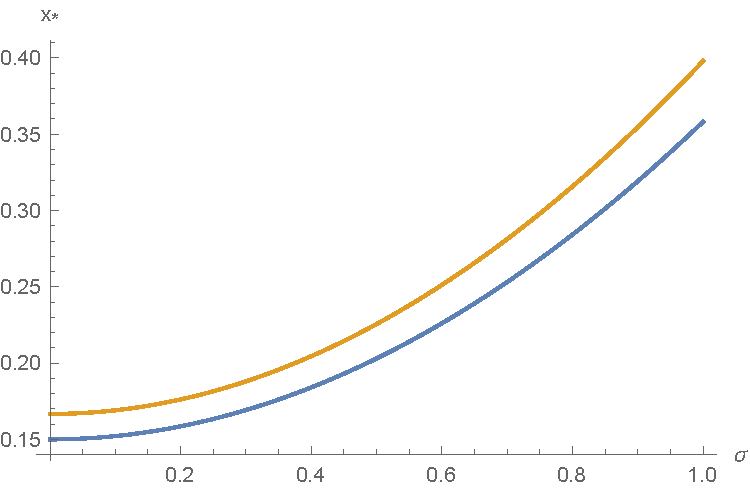
\includegraphics[width=0.45\textwidth]{Prob1_CapOpt/xopt_mu-7.pdf}}
			\subfigure[$\mu=0.03$]{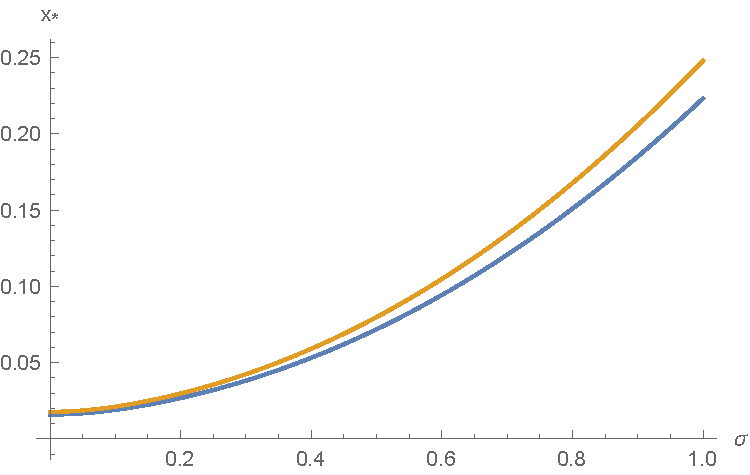
\includegraphics[width=0.45\textwidth]{Prob1_CapOpt/xopt_mu03.pdf}}
			\end{subfigmatrix}
			\caption{Threshold value with respect to the benchmark model (orange) and the capacity optimized model (blue), considering volatility $\sigma \in [0.0001, 1]$.}
			\label{fig:sigm}
\end{figure}

Regarding the drift parameter $\mu$ we obtained that the threshold values do not have a monotonic behaviour, either for smaller or bigger values of volatility. As showed in Figure \ref{fig:mu}, the smallest value of demand level necessary to invest is observed at the stationary point when $\mu=\sigma^2/2$.

\begin{figure}[!htb]
	\begin{subfigmatrix}{2}
		\subfigure[$\sigma=0.0001$]{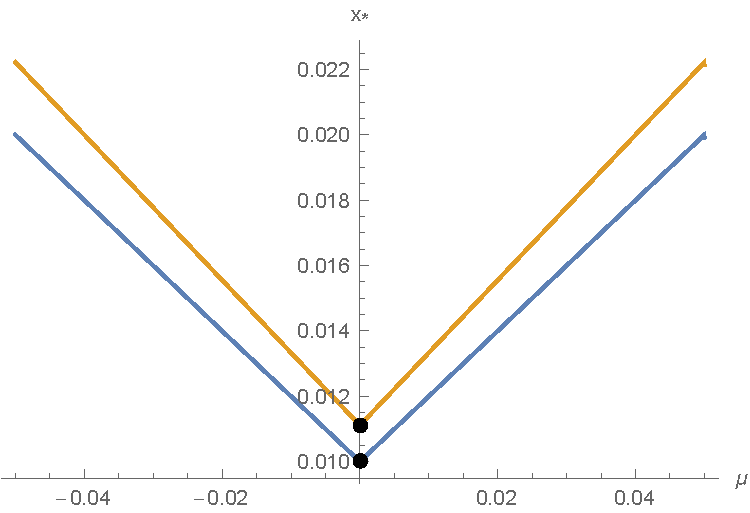
\includegraphics[width=0.45\textwidth]{Prob1_CapOpt/xopt_sigma0001.pdf}}
		\subfigure[$\sigma=0.3$]{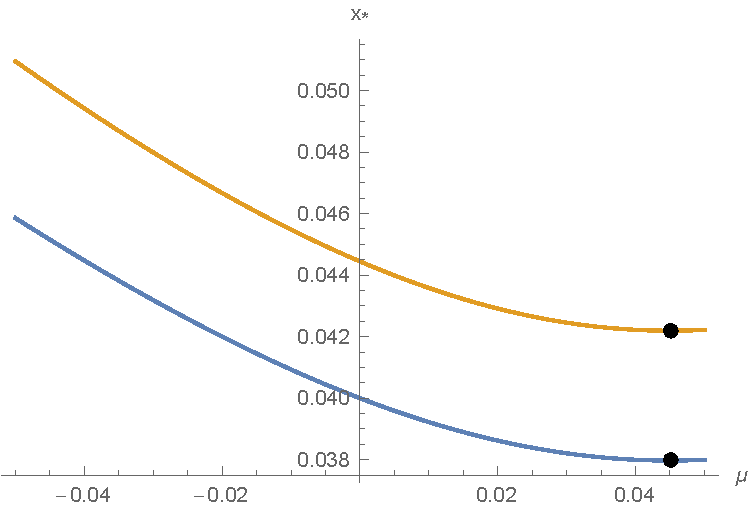
\includegraphics[width=0.45\textwidth]{Prob1_CapOpt/xopt_sigma3.pdf}}
	\end{subfigmatrix}
	\caption{Threshold value with respect to the benchmark model (orange) and the capacity optimized model (blue), considering drift $\mu \in [-r, r]$ and corresponding stationary point $\sigma^2/2$ (black).}
	\label{fig:mu}
\end{figure}

On Figure \ref{fig:td} we observe the behaviour of both threshold levels regarding the two other parameters, sensibility level $\delta$ and innovation level $\theta$. We have that the threshold levels increase with $\delta$ and decrease with $\theta$.

\begin{figure}[!htb]
	\begin{subfigmatrix}{2}
	\subfigure[$\delta \in ( 0,10 )$ ]{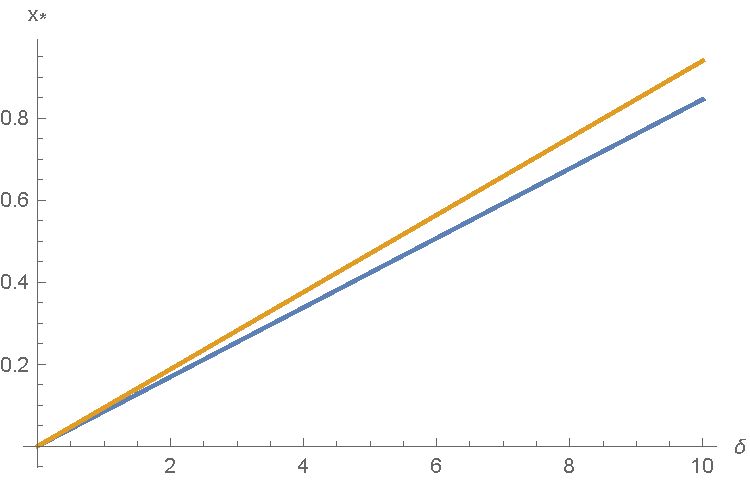
\includegraphics[width=0.45\textwidth]{Prob1_CapOpt/xopt_deltavar.pdf}}
	\subfigure[$\theta \in (\alpha K=1,50)$]{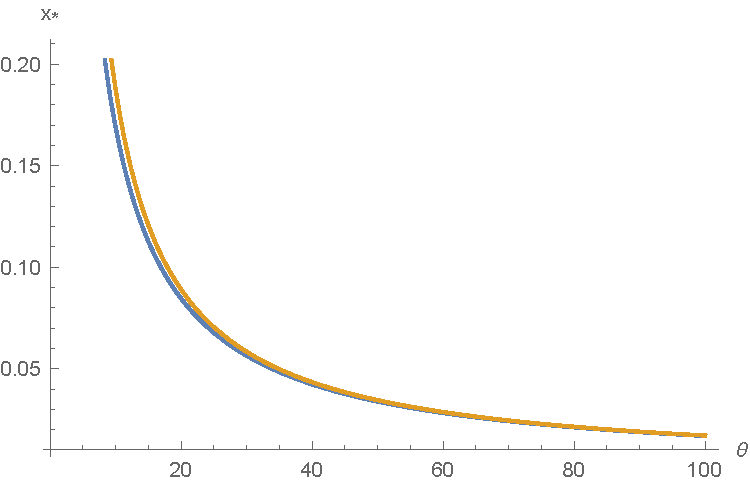
\includegraphics[width=0.45\textwidth]{Prob1_CapOpt/xopt_thetavar.pdf}}
	\end{subfigmatrix}
\caption{Threshold value with respect to the benchmark model (orange) and the capacity optimized model (blue), regarding sensibility parameter $\delta$ and innovation level $\theta$.}
\label{fig:td}
\end{figure}



Now we analyse optimal capacity level $K^*_C$, that is given by evaluating $K^*$ as defined in \eqref{} on demand level $x^*_C$, as done in \cite{huis:cap}. Its expression is given by
$$K^*_C=\frac{2 \sigma ^2 \theta}{\alpha \left(\sigma ^2 \left(\sqrt{\frac{4 \mu ^2}{\sigma ^4}-\frac{4 \mu }{\sigma ^2}+\frac{8 r}{\sigma ^2}+1}+3\right)-2 \mu \right)}.$$\\
\textbf{Proposition:}
Optimal capacity level $K^*_C$ increases with $\mu$, $\sigma$ and $\theta$ and decreases with $r$ and $\alpha$.

\textbf{Proof:}
The relation between $K^*_C$ and $\theta$, $r$ or $\alpha$ comes immediately by observing $K^*_C$ expression.

Now, regarding drift parameter we obtain that
 \begin{align*}
\frac{\partial K^*_C(\mu)}{\partial \mu}=
\frac{4 \theta \left(\sigma ^2 \left(\sqrt{\frac{4 \mu ^2}{\sigma ^4}-\frac{4 \mu }{\sigma ^2}+\frac{8 r}{\sigma ^2}+1}+1\right)-2 \mu \right)}{\alpha \sqrt{\frac{4 \mu ^2}{\sigma ^4}-\frac{4 \mu }{\sigma ^2}+\frac{8 r}{\sigma ^2}+1} \left(\sigma ^2 \left(\sqrt{\frac{4 \mu ^2}{\sigma ^4}-\frac{4 \mu }{\sigma ^2}+\frac{8 r}{\sigma ^2}+1}+3\right)-2 \mu \right)^2}>0.
\end{align*}
Since from
\begin{align}
\label{cond2}
\sigma ^2 \left(\sqrt{\frac{4 \mu ^2}{\sigma ^4}-\frac{4 \mu }{\sigma ^2}+\frac{8 r}{\sigma ^2}+1}+1\right)-2 \mu\geq0 
& \Leftrightarrow
\frac{4 \mu ^2}{\sigma ^4}-\frac{4 \mu }{\sigma ^2}+\frac{8 r}{\sigma ^2}+1 \geq \left( \frac{2 \mu}{\sigma^4}-1 \right)^2=\frac{4 \mu ^2}{\sigma ^4}-\frac{4 \mu }{\sigma ^2}+1 \\
& \Leftrightarrow
\frac{8 r}{\sigma ^2}\geq 0, \nonumber
\end{align}
which is true for $\forall r\geq 0$, and from \eqref{condd1} we obtain that both denominator and numerator are positive, from which the result comes.

Regarding volatility parameter we obtain that
 $$    \frac{\partial K^*_C(\sigma)}{\partial \sigma}= 
\frac{8 \theta \left(2 \mu ^2-\mu  \sigma ^2 \left(\sqrt{\frac{4 \mu ^2}{\sigma ^4}-\frac{4 \mu }{\sigma ^2}+\frac{8 r}{\sigma ^2}+1}+1\right)+2 r \sigma ^2\right)}{\alpha \sigma  \sqrt{\frac{4 \mu ^2}{\sigma ^4}-\frac{4 \mu }{\sigma ^2}+\frac{8 r}{\sigma ^2}+1} \left(\sigma ^2 \left(\sqrt{\frac{4 \mu ^2}{\sigma ^4}-\frac{4 \mu }{\sigma ^2}+\frac{8 r}{\sigma ^2}+1}+3\right)-2 \mu \right)^2}>0$$

From \eqref{demo} we obtain that the denominator is positive and from \eqref{condd1} and \eqref{cond2} that the denominator is positive for $\forall r\geq0$, from which the result holds.
\begin{flushright}
	$\square$
\end{flushright}


Considering some numerical approximations, we observe, on Figure \ref{fig:k1}, that $K^*_C$ increases with both drift and volatility. Note that, regarding the drift parameter, the growth is barely noticeable for negative values of $\mu$, but then it turns to be logarithmic. FINANCIAL INTERPRETATION? This seems to be related with the fact that for small drift values, the future expected demand value is smaller that for positive drift values. Recall that the demand process evolves accordingly to a GBM and its expected value at time $t$ is given by $\mathds{E}^{X_0=x_0} [X_t]=x_0 e^{\mu t}$.

\begin{figure}[!htb]
	\begin{subfigmatrix}{2}
		\subfigure[$\mu \in ( -r,r )$ ]{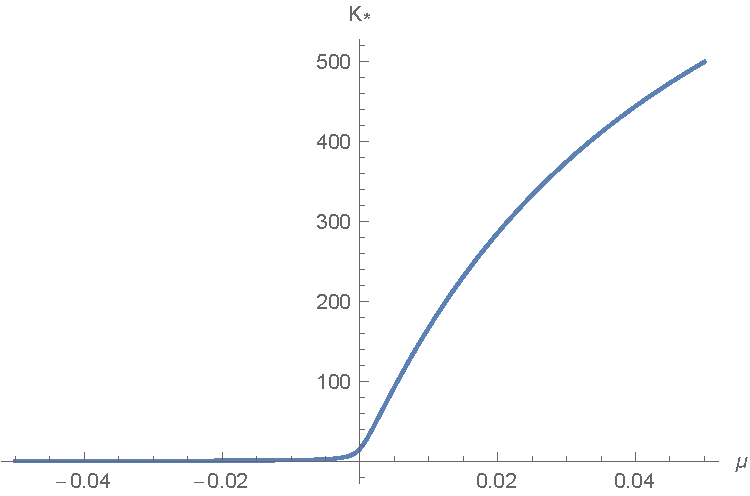
\includegraphics[width=0.45\textwidth]{Prob1_CapOpt/koptx_sigma005.pdf}}
		\subfigure[$\sigma \in (0,1)$]{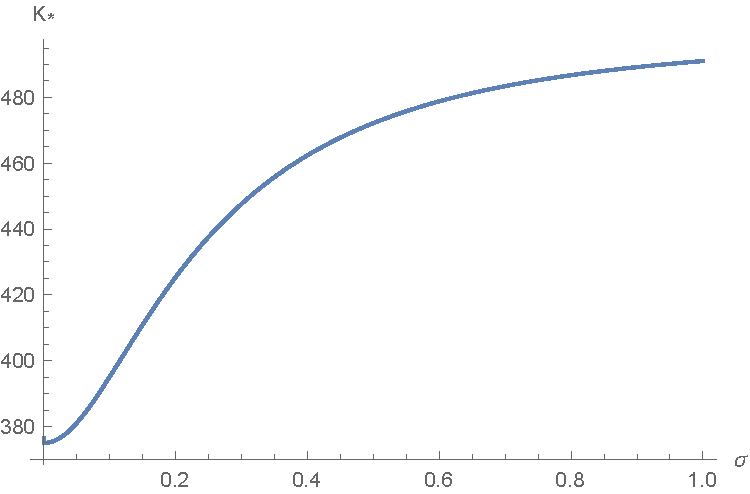
\includegraphics[width=0.45\textwidth]{Prob1_CapOpt/koptx_mu03.pdf}}
	\end{subfigmatrix}
	\caption{Optimal capacity regarding the threshold value $x^*_C$.}
	\label{fig:k1}
\end{figure}

Regarding discount rate $r$ and sensibility parameter $\alpha$, we have on Figure \ref{fig:k2} that $K^*_C$ decreases with them, as expected.
 
\begin{figure}[!htb]
	\begin{subfigmatrix}{2}
		\subfigure[$ r \in ( \mu, 1 )$]{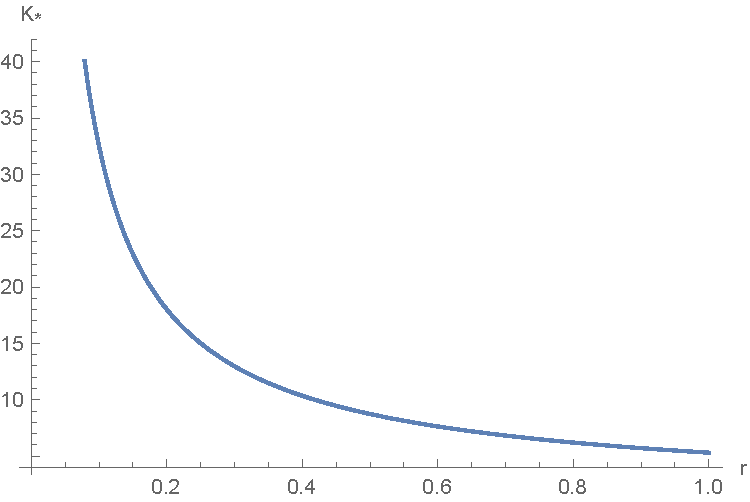
\includegraphics[width=0.45\textwidth]{Prob1_CapOpt/koptx_varr.pdf}}
		\subfigure[$ \alpha \in (0,1)$]{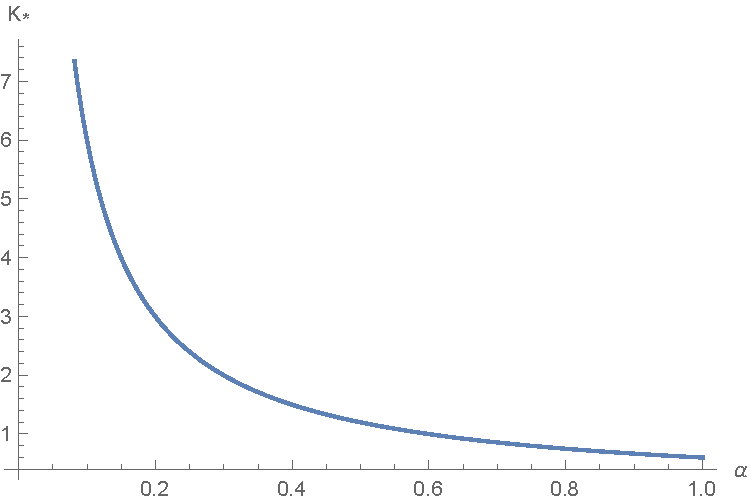
\includegraphics[width=0.45\textwidth]{Prob1_CapOpt/koptx_varalfa.pdf}}
	\end{subfigmatrix}
	\caption{Optimal capacity regarding the threshold value $x^*_C$.}
	\label{fig:k2}
\end{figure}









\subsection{R\&D and Capacity Optimization Model}
\label{subsec:RDcap1}

As stated in section \ref{prob1max}, we are not able to solve analytically the polynomial presented in \eqref{} for every value $\gamma \in (0,1)$. However we considered some numerical approximations, using software \textit{Mathematica} and its function \texttt{Solve}. For the effect, we considered 
\begin{itemize}
	\item $r=0.05$;
	\item $F(X)=10$;
	\item $\gamma \in (0,1]$ incremented by 0.05.
\end{itemize}

Following results are implemented on script \texttt{RVopt.nb}.


\begin{figure}[!htb]
	\centering
	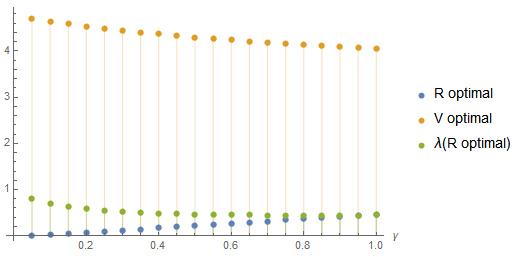
\includegraphics[width=0.6\textwidth]{Prob1_MaxProb/RVlambda_opt05.PNG}
	\caption{Optimal values of $R$ and $V(X)$ for fixed values of $F$ and $r$}
\end{figure}

We obtain that, although the optimal investment $R$ grows with exponent $\gamma$, the value function for the respective optimal $R$ decreases with exponent $\gamma$ (and in a different way from the decreasing of $\lambda(R)$). We get that the smaller value of $V(X)$ is approximately 4.05, corresponding to the optimal investment level $R=1$ and $\lambda(R)=0.45$ and the biggest value of $V(X)$ is approximately 4.69, corresponding to the optimal investment level $R=0.014$ and $\lambda(R)=0.05$















